\scanpage{86}
\mspage{85}
\mspage{\handwritten{18}}
\mspage{\deleted{\handwritten{16}}}
\margin{\handwritten{\figure{\begin{tikzpicture}[x=.12cm,y=.12cm]
\draw[line width=.6pt] (0,1.55)--(-.04,1.25);
\draw[line width=.4pt] (-.08,.8)--(-.12,-.2);
\end{tikzpicture}}}}
2.7\rlap{\handwritten{\begin{tikzpicture}[baseline=0cm,x=1cm,y=1cm]\draw[thin] (.04,.02)--(.05,.27);\end{tikzpicture}}}. \handwritten{\uline}{Classifying topos of a \inserted{\handwritten{pro-}}\handwritten{\begin{tikzpicture}[baseline=0cm,x=1cm,y=1cm]\draw[thin] (0,-.15)..controls (.05,.08) and (.1,.18)..(.35,.2)--(.8,.24);\end{tikzpicture}}group\handwritten{.} \deleted{profinite}.}

\handwritten{\begin{tikzpicture}[baseline=0cm]\fill (0,0) circle (.018cm);\end{tikzpicture}}\handwritten{2.7.1} Let $\inserted{\handwritten{\underline}{G}=}(G_i)_{i\handwritten{\in}I}$ be a projective syst\rlap{p}e\rlap{e}m \deleted{strict} of groups, with $G_i,I\handwritten{\in}\handwritten{\underline}{U}$. One assumes the projective system \handwritten{\uline}{strict}, i.e. the transition morphisms $G_j\handwritten{\to}G_i$ surjective. \margin{\handwritten{\figure{\begin{tikzpicture}[x=.3cm,y=.3cm]
\draw (0,.15) .. controls (.2,-.05) and (.4,-.25) .. (.65,-.2);
\end{tikzpicture}}}}If $E$ is a s\rlap{s}e\rlap{n}t, one \deleted{says that $\handwritten{\underline}{G}$ \handwritten{\uline}{acts} on $E$} \deleted{if} calls an \handwritten{\uline}{action of} $\handwritten{\underline}{G}$ \handwritten{\uline}{on} $E$\inserted{(on the left, say\unsure{\rlap{p}\handwritten{)}|)\handwritten{)}}}\handwritten{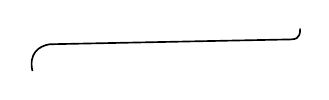
\begin{tikzpicture}[baseline=0cm,x=1cm,y=1cm]\draw[semithick] (0,-.17)..controls (-.05,.05) and (.08,.15)..(.22,.17)--(3.2,.23)..controls (3.35,.23) and (3.4,.23)..(3.4,.37);\end{tikzpicture}} the following structure: a) a family $(E_i)_{i\handwritten{\in}I}$ of subsets of $E$, with union $E$; b) for every $i\handwritten{\in}I$, an action of the group $G_i$ on the set $E_i$ ; one assumes moreover these data subject to the following condition: for $j\handwritten{\geq}i$, $E_i$ is the subset of $E_j$ consisting of the elements fixed under the kernel group of $G_j\handwritten{\to}G_i$. One says \inserted{\handwritten{also}}\handwritten{\begin{tikzpicture}[baseline=0cm,x=1cm,y=1cm]\draw[thin] (0,-.15)..controls (.05,.12) and (.2,.18)..(.48,.22)..controls (.7,.25) and (.82,.28)..(.82,.37);\end{tikzpicture}} that \handwritten{\uline}{$G$ acts on} $E$ (on the left) if one has given\deleted{\unsure{s|x}} oneself an action of $G$ on $E$ (on the left).

The sets $\handwritten{\in}\handwritten{\underline}{U}$ endowed with an action of $\handwritten{\underline}{G}$ form a category in an obvious way. One observes at once, thanks to Giraud's criterion, that this category is a \inserted{\handwritten{$\underline{U}$-}}\handwritten{\begin{tikzpicture}[baseline=0cm,x=1cm,y=1cm]\draw[thin] (0,-.15)..controls (.05,.12) and (.2,.18)..(.48,.22)..controls (.7,.25) and (.82,.28)..(.82,.37);\end{tikzpicture}}topos. One denotes it $B_{\handwritten{\underline}{G}}$ and one call\deleted{l}s it the \handwritten{\uline}{classifying topos of $G$}. When $I$ admits an \deleted{\unsure{fin|fix}} initial object $i_{\unsure{\rlap{$a$}o|o|0}}$, putting $G=G_{i_o}$, one recovers the classifying topos of 2.3.
\margin{\handwritten{\figure{
\begin{tikzpicture}[baseline]
\draw[rotate=18] (0,0) ellipse (1.05 and .43);
\node[rotate=18] at (0,0) {new line};
\end{tikzpicture}}}}

\handwritten{\figure{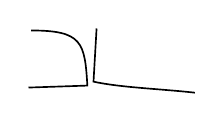
\begin{tikzpicture}[x=.65cm,y=.5cm]
\draw[line width=.6pt] (-1.1,.8) .. controls (-.1,.8) and (-.05,.5) .. (0,-.6) -- (-1.15,-.65);
\draw[line width=.6pt] (.18,.85)--(.12,-.5) .. controls (.65,-.65) and (1.4,-.68) .. (2.1,-.78);
\end{tikzpicture}}}
\inserted{\handwritten{2.7.2.}} A\unsure{\rlap{a}n|\rlap{\raisebox{-.2ex}{n}}n}other important example is that where the groups $G_i$ are finite, so that
\[
G=\underset{\handwritten{\longleftarrow}}{\lim}G_i
\]
is\deleted{\unsure{n|x}} a compact totally disconnected topological group, or \handwritten{\uline}{pro\rlap{f}\handwritten{f}inite group}. A\unsure{\rlap{a}n|\rlap{\raisebox{-.2ex}{n}}n} action of $\handwritten{\underline}{G}$ on $E$ then amounts to an action of $G$ on $E$ which is continuous, or what amounts to the same thing, such that the stabilizer of every point of $E$ is an open subgroup of $G$. The classifying topos $B_{\handwritten{\underline}{G}}$ will also be denoted $B_G$, where,of course, $G$ must be considered as endowed with its profinite topology.

\handwritten{2.7.3.} It is easy to verify,\deleted{that} using the remarks of 2.6, that the topos $B_{\handwritten{\underline}{G}}$ defined by a strict projective system \deleted{of} $\handwritten{\underline}{G}=(G_i)_{i\handwritten{\in}I}$ of groups is equivalent to a topos of the form $\handwritten{\hat}{C}$ only if this projective system is essentially constant; in the case of a profinite group, this means that this group is in fact finite.
